\documentclass{article}
%%%%%%% PACKAGES %%%%%%%%
\usepackage[utf8]{inputenc}
\usepackage[margin=3cm]{geometry}
\usepackage{graphicx}

\title{Software Engineering Project Architecture}
\author{Muhammad Azeem Haider $\mid$ Ali Asghar Yousuf \\
    Muhammad Shahid Mehmood $\mid$ Musab Sattar}
\date{\today}

\begin{document}

\maketitle

\section*{Introduction}

Thekedaar hatao is an application that aims to ease the process of building
your dream home. It provides the users with features that makes the building
process smoother and easier overall for the user of the application. The
calculator on the application, will provide you with an estimated amount of
cement, cinder blocks, sand, and other such raw materials that are essential
while building your house. In addition, the application will help cater the
dreamers by having a forum where people can communicate about the problems that
have arisen and how they tackled them. Advice threads and asking for help will
be carried out on the forum. Since you can never be sure of how much material
you exactly need, there is always a (+ or -)5\% chance of having extra
material, you can also sell this to other users on the app through a buy and
sell section. For individuals wanting to have a communication privately, the
application will also provide an opportunity to privately chat with someone
registered on the application.

\section*{Requirements}

\subsubsection*{Functional}

\subsubsection*{Non-Functional}

\begin{enumerate}

    \item \textbf{Performance}

          The application will run smoothly on all devices supporting IOS 15 (and above)
          or Android 10 (and above). The application would not be resource intensive thus
          the performance would be enhanced.

    \item \textbf{Aesthetic}

          The aesthetic of the application will be developed in a way where it will make
          it easy for the users of the application to use it efficiently. The different
          features of the application will be inter-connected in a manner that will make
          the application a useful addition.

    \item \textbf{Usability}

          The mobile application will be usable in the sense that it will be easy for
          people of all ages to use the application for their benefit. The calculator,
          forum, marketplace, and chat messaging will all be easy to use.

    \item \textbf{Compatability}

          The application will be compatible with all mobile phones supporting the
          recommended operating system.

    \item \textbf{Reliability}

          The application will be reliable in the sense that it will not crash for users
          when they are using it. The application will also be reliable as it will always
          provide the perfect solution to the best of the applications knowledge.

    \item \textbf{Security}

          The user details submitted at the time of sign up to the application will be
          secure and will not be released to the public at any time.

\end{enumerate}

\section*{Use Cases}
\centering
\begin{figure}[!h]
    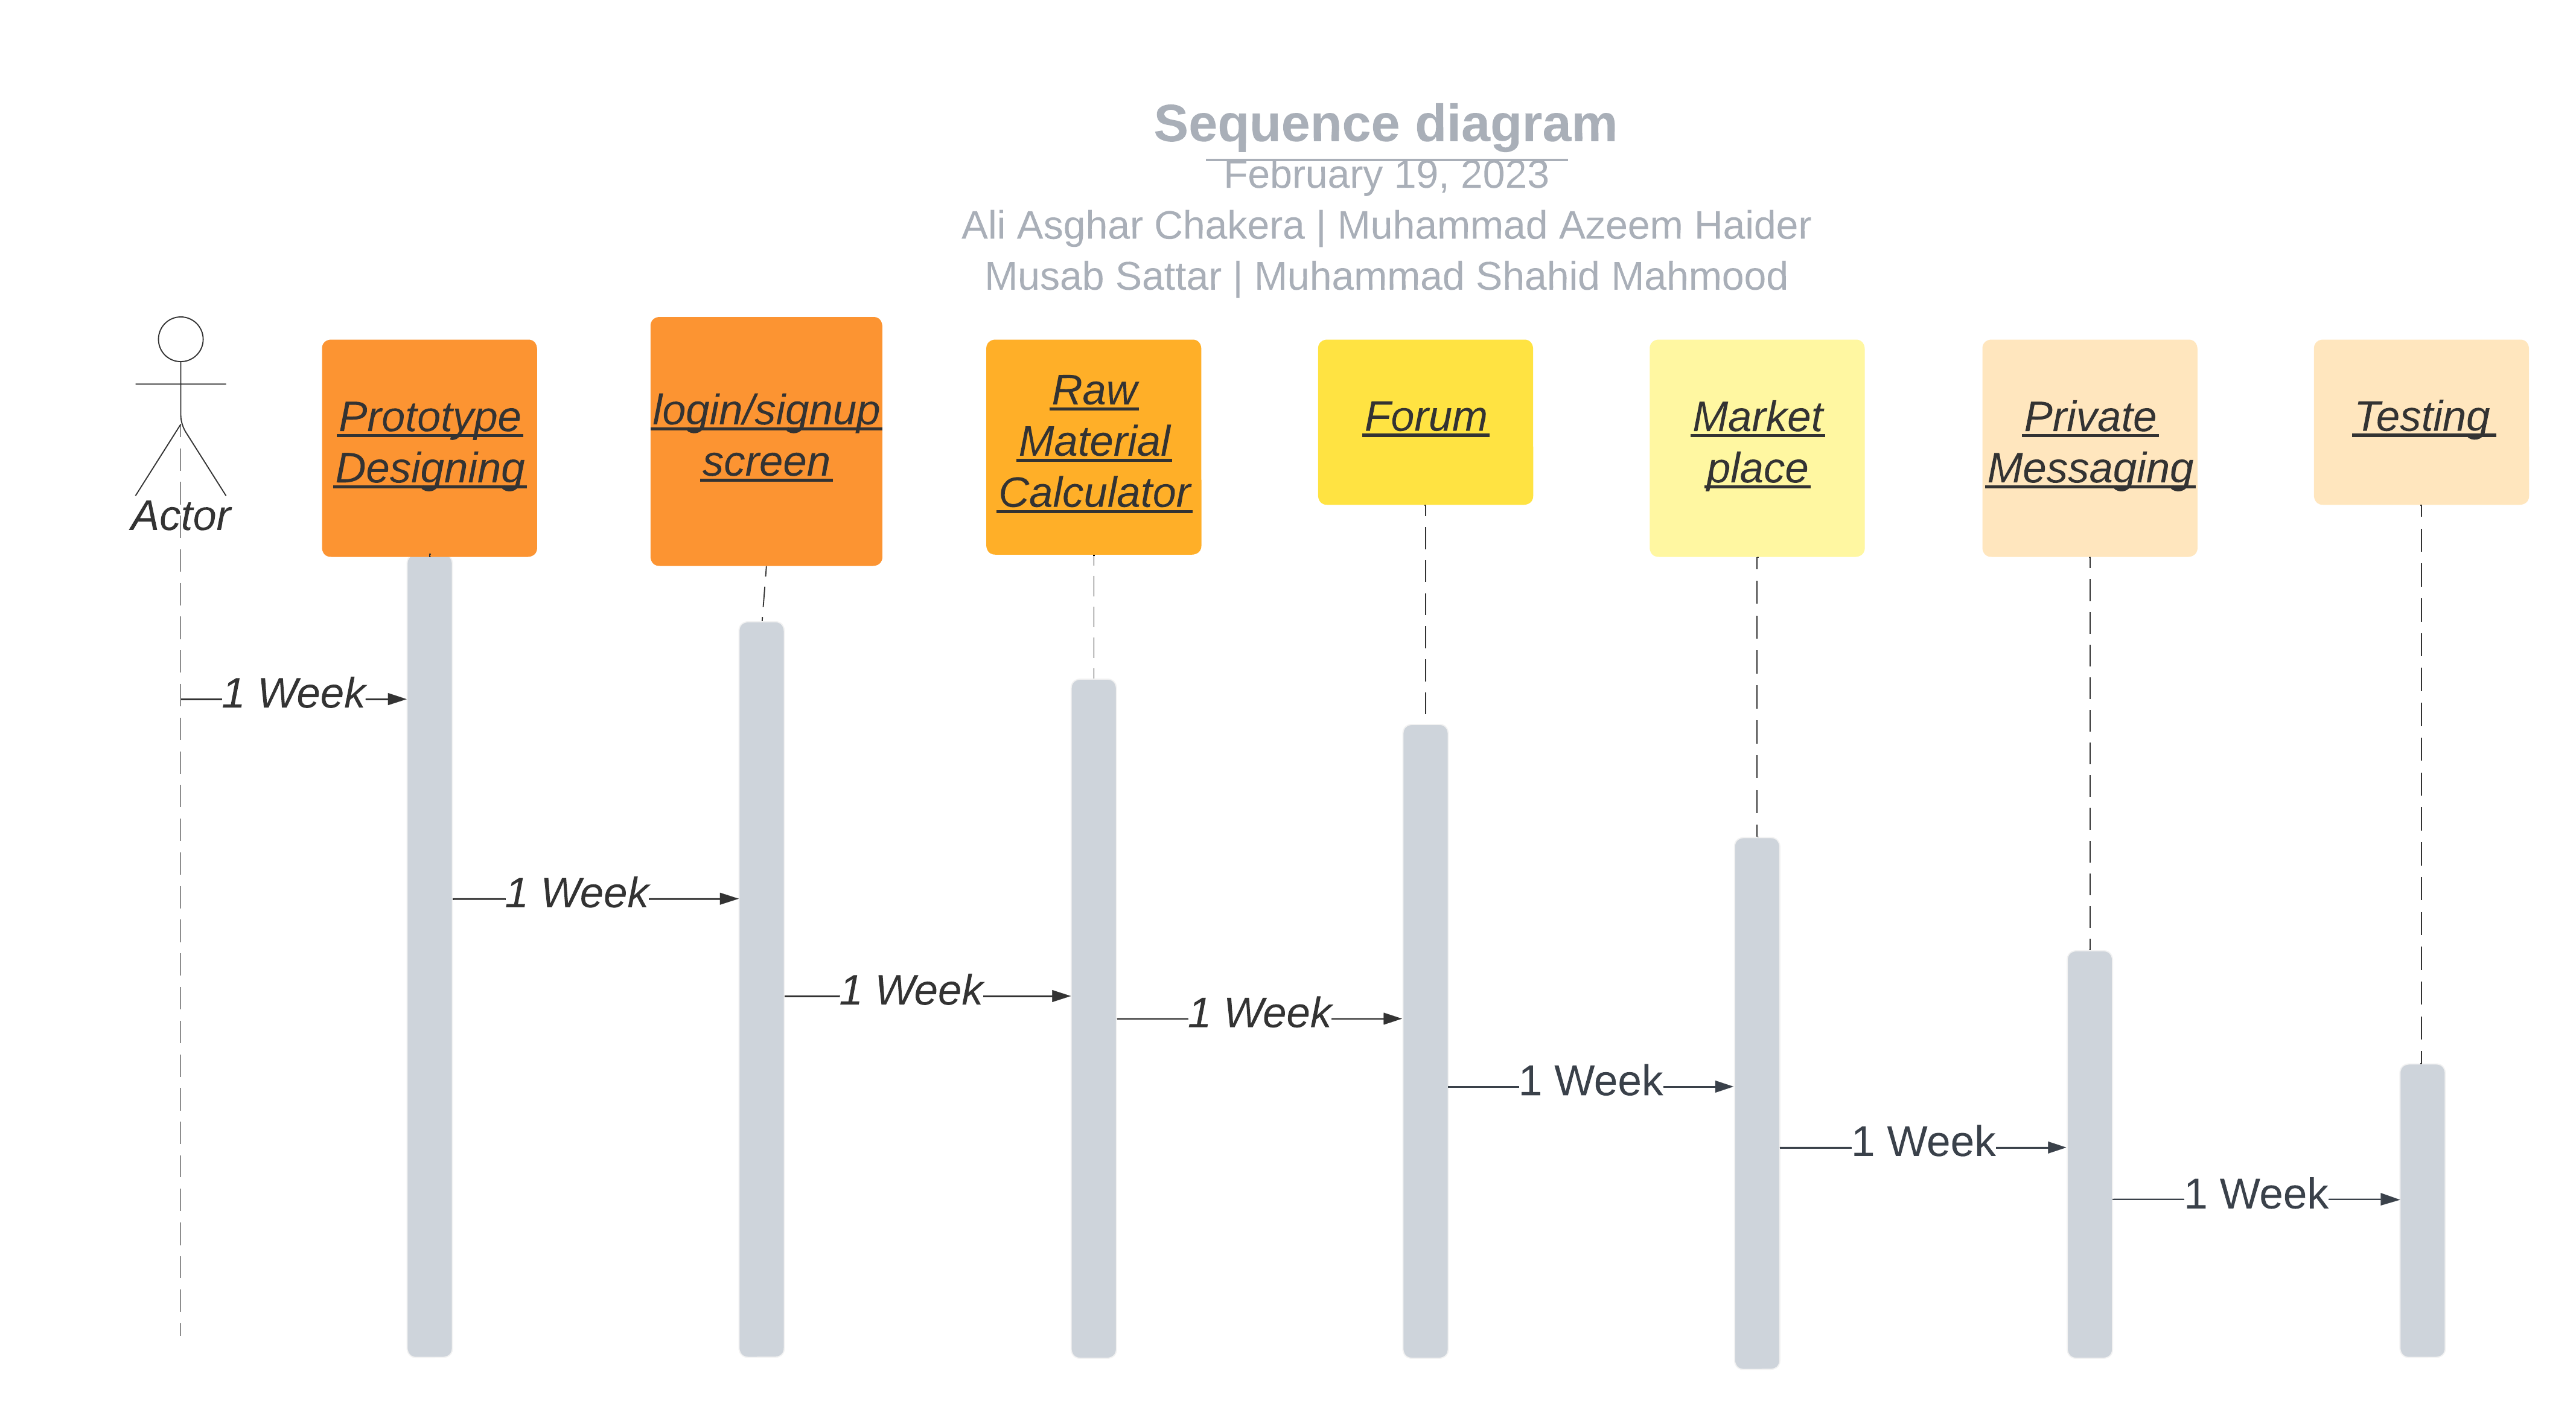
\includegraphics[width=1\linewidth]{Sequence diagram.png}
    \caption{usecase}
    \label{fig:seq}
\end{figure}


\subsubsection*{Explanation}

\section*{Class Diagrams}

\section*{Sequence Diagrams}
\centering
\begin{figure}[!h]
    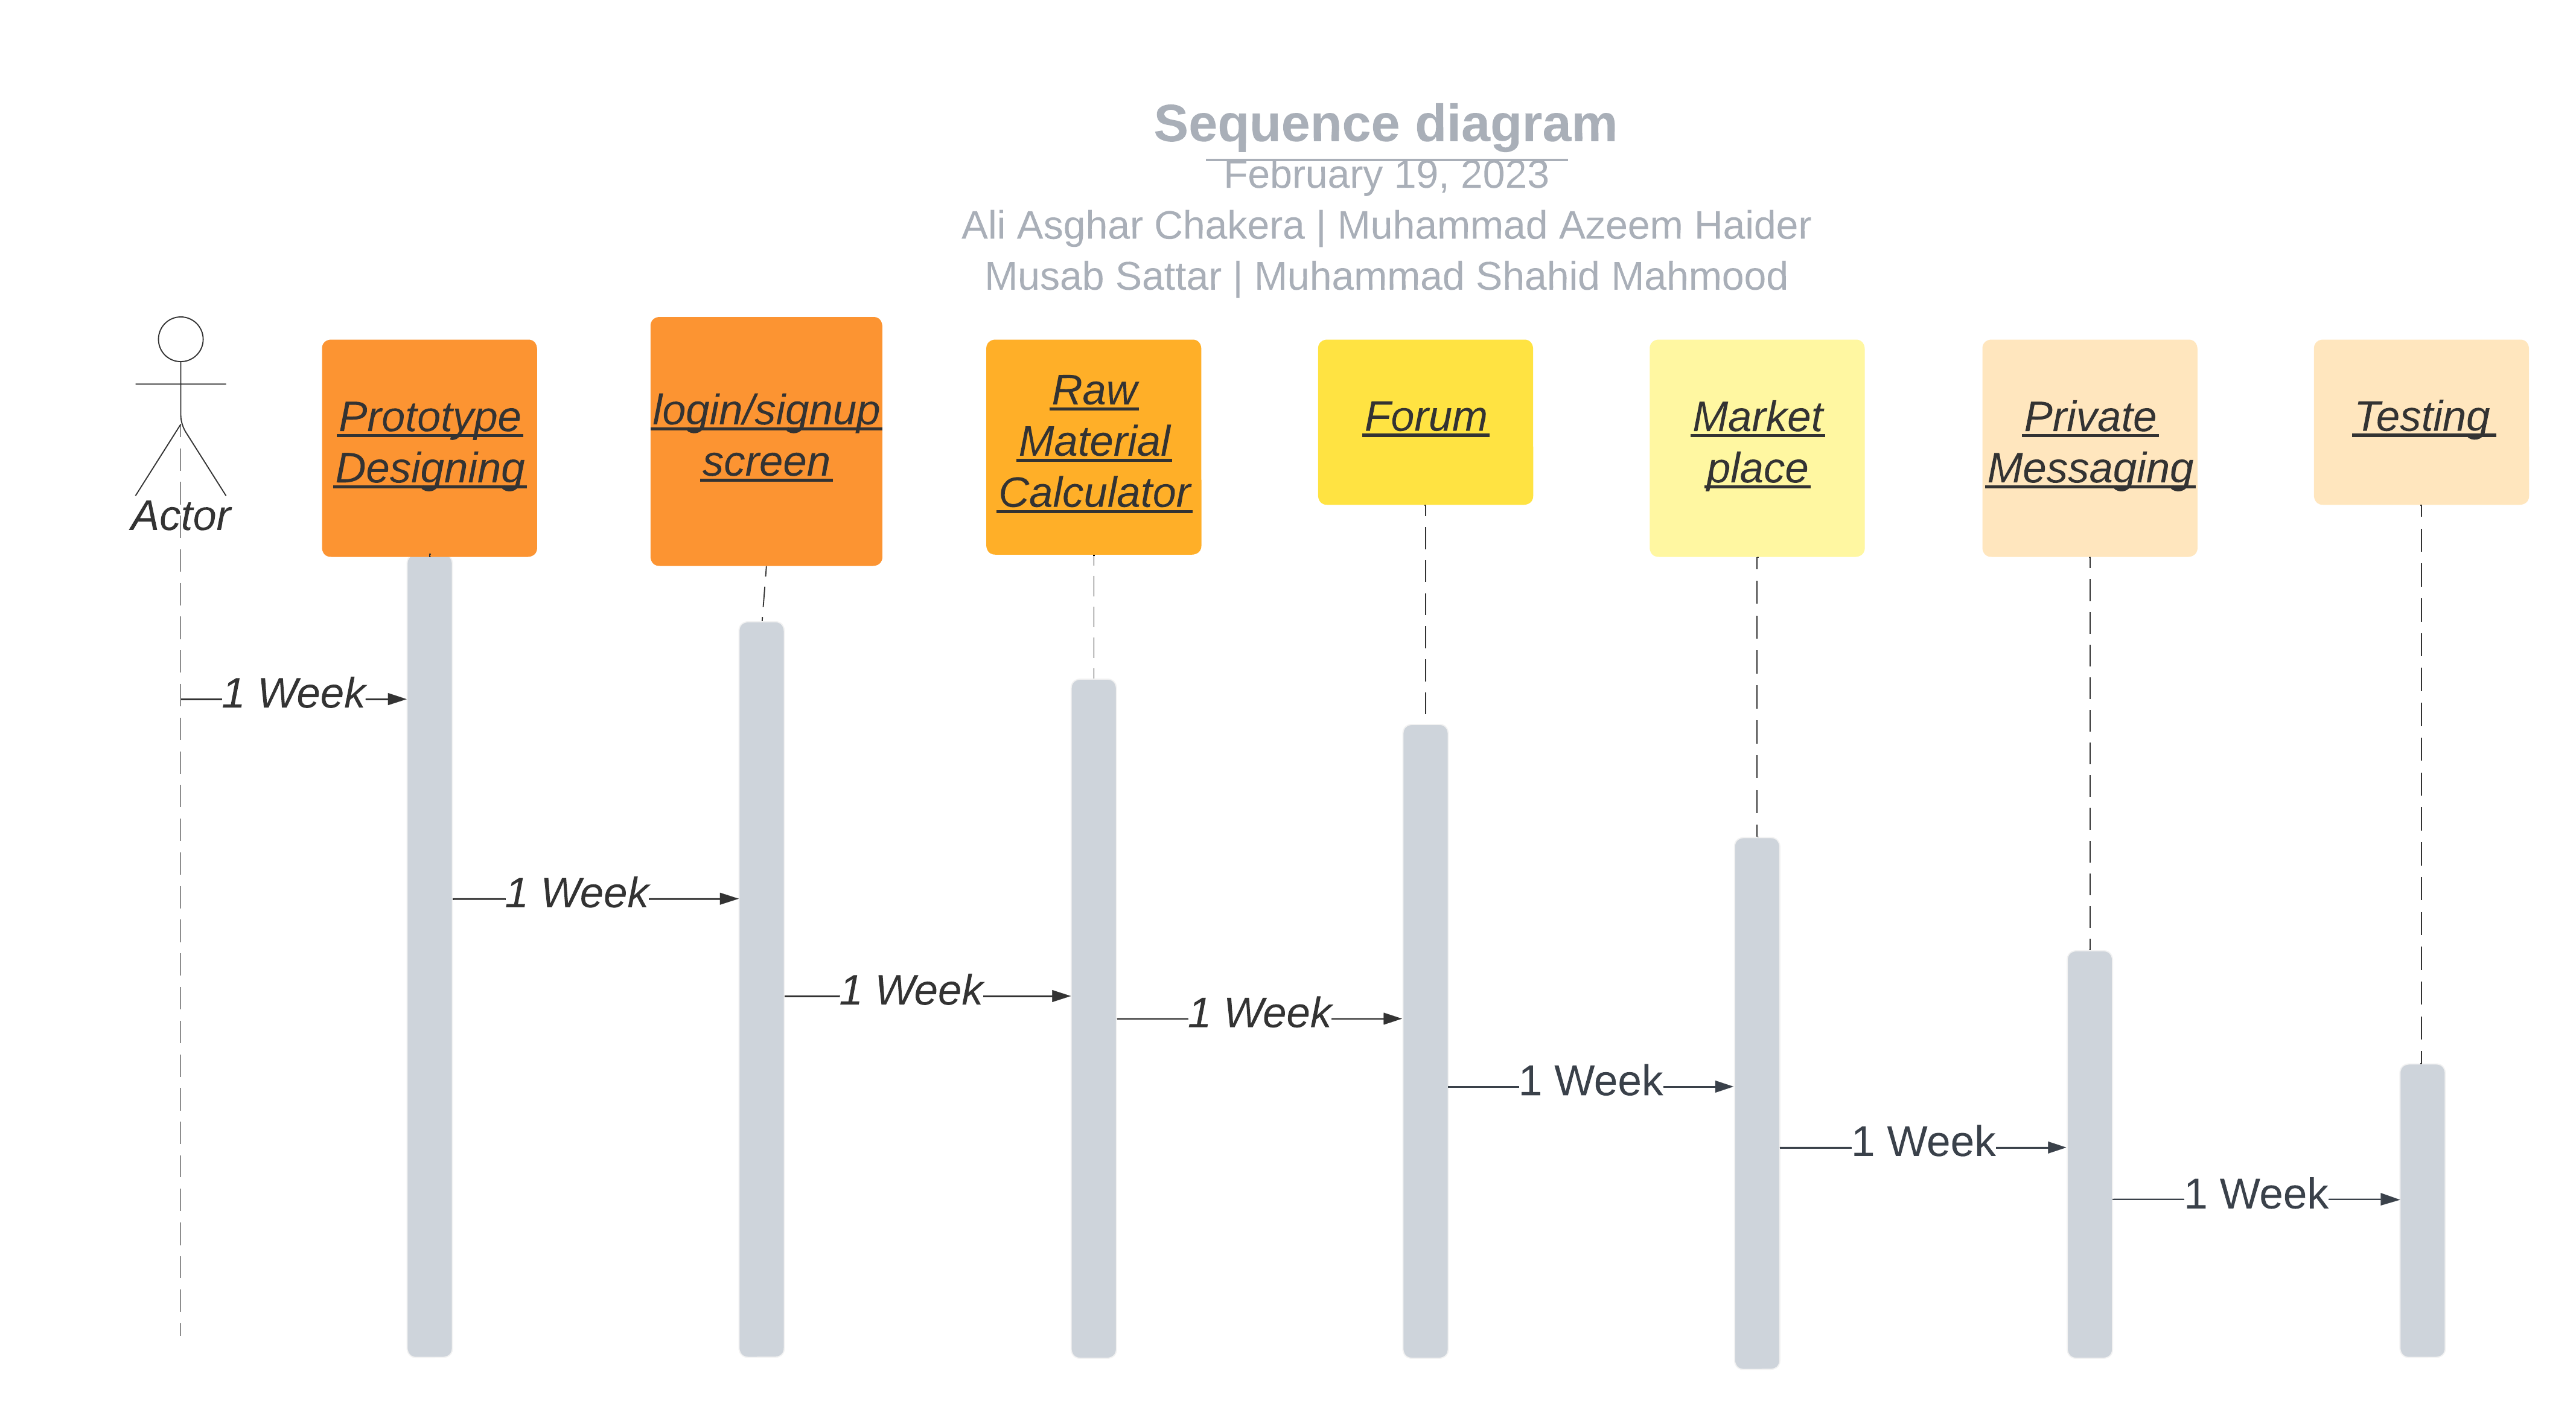
\includegraphics[width=1\linewidth]{Sequence diagram.png}
    \caption{Sequence Diagram}
    \label{fig:seq}
\end{figure}

\end{document}